\documentclass[pdftex,12pt,a4paper]{article}

\usepackage[utf8]{inputenc}
\usepackage[T1]{fontenc}
%\usepackage{fontspec}
%\usepackage{xunicode}
\usepackage[frenchb]{babel}
\usepackage{color}
\usepackage[usenames,dvipsnames,svgnames,table]{xcolor}
\usepackage{lmodern}
\usepackage{lastpage}
\usepackage[pdftex]{graphicx}
\usepackage{fancyhdr}
\usepackage{geometry}
%\usepackage{layout}
%\usepackage{setspace}
%\usepackage{soul}
%\usepackage{ulem}
%\usepackage{eurosym}
%\usepackage{bookman}
%\usepackage{charter}
%\usepackage{newcent}
%\usepackage{mathpazo}
%\usepackage{mathptmx}
\usepackage{hyperref}
%\usepackage{verbatim}
\usepackage{fancyvrb}
\usepackage{titling}
%\usepackage{moreverb}
%\usepackage{listings}
%\usepackage{wrapfig}
%\usepackage{colortbl}
%\usepackage{amsmath}
\usepackage{amssymb}
%\usepackage{mathrsfs}
%\usepackage{asmthm}
%\usepackage{makeidx}
\usepackage{tabularx}
\usepackage{float}
\usepackage{lastpage}


\usepackage{listings}	   % Code insertion
\lstdefinestyle{customstyle}{
    basicstyle=\footnotesize,
    breakatwhitespace=false,
    breaklines=true,
    captionpos=b,
    keepspaces=true,
    tabsize=4,
    frame=single
}
\lstset{style=customstyle}


\geometry{top=3cm, bottom=2.5cm, left=2cm, right=2cm}
\setcounter{tocdepth}{3}

%%%%%%%   MAKE TITLE   %%%%%%%%%%%%%%%%%%%%%%%%%%%%%%%%%%%%%
\title{Projet Système de feux tricolores}
\author{Adrien Garandel \and Ran Bao \and Franck Boncler \and Jérémy Bardon}
\pretitle{\begin{center}%
\rule{\textwidth}{1.6pt}\vspace*{-\baselineskip}\vspace*{2pt} %
\rule{\textwidth}{0.4pt}\par\Huge}
\posttitle{\par\vspace*{-0.6\baselineskip}%
\rule{0.3\textwidth}{0.2pt}%
\vspace*{-0.5\baselineskip}%
\end{center}}

\preauthor{\begin{center}
\LARGE \lineskip 0.5em%
\begin{tabular}[t]{c}}
\postauthor{\end{tabular}\par\end{center}}

\predate{\begin{center}\large}
\postdate{\par%
\rule{\textwidth}{0.4pt}\vspace*{-\baselineskip}%
\vspace*{3.2pt} %
\rule{\textwidth}{1.6pt}%
\vspace*{\baselineskip}\end{center}}

\makeatletter
\let\doctitle\@title
\let\docauthor\@author
\let\docdate\@date
\makeatother
%%%%%%%%%%%%%%%%%%%%%%%%%%%%%%%%%%%%%%%%%%%%%%%%%%%%%%%%%%%%

%%%%%%  EN-TETE / PIED-PAGE %%%%%%%%%%%%%%%%%%%%%%%%%%%%%%%%
\pagestyle{fancy}
\setlength{\headheight}{15pt}
\fancyhead{}
\fancyfoot{}
\fancyhead[L]{\leftmark}
\fancyhead[R]{\doctitle}
\fancyfoot[L]{Adrien Garandel, Ran Bao, Franck Boncler, Jérémy Bardon}
\fancyfoot[R]{\thepage/\pageref{LastPage}}

\fancypagestyle{plain}{
	\fancyhf{}
	\fancyfoot[R]{\thepage/\pageref{LastPage}}
	\renewcommand{\headrulewidth}{0pt}
	\renewcommand{\footrulewidth}{0.5pt}
}

\renewcommand{\footrulewidth}{0.5pt}
\renewcommand{\headrulewidth}{0.5pt}
%%%%%%%%%%%%%%%%%%%%%%%%%%%%%%%%%%%%%%%%%%%%%%%%%%%%%%%%%%%%

\renewcommand{\FrenchLabelItem}{\space\textbullet}

\hypersetup{
    bookmarks=true,
    unicode=false,
    pdftitle={\doctitle},
    pdfauthor={Adrien Garandel, Ran Bao, Franck Boncler, Jérémy Bardon},
    pdfnewwindow=true,
    colorlinks=true,
    linkcolor=black,
    citecolor=black,
    filecolor=black,
    urlcolor=black
}

\begin{document}

\maketitle
\tableofcontents
\newpage

%%%%%%%%%%%%%%%%%%%%%%%%%%%%%%%%%%%%%%%%%%%%
\section{Partie 1 - Deux feux synchronisés}
%%%%%%%%%%%%%%%%%%%%%%%%%%%%%%%%%%%%%%%%%%%%
Dans cette partie, on s'intéresse à la synchronisation de deux feux tricolores. On utilise pour cela des réseaux de Pétri et le logiciel Roméo.

%%%%%%%%%%%%%%%%%%%%%%%
\subsection{Questions 1 et 2}
%%%%%%%%%%%%%%%%%%%%%%%
Feux non synchronisés et non temporises

\begin{figure}[H]
	\centering
	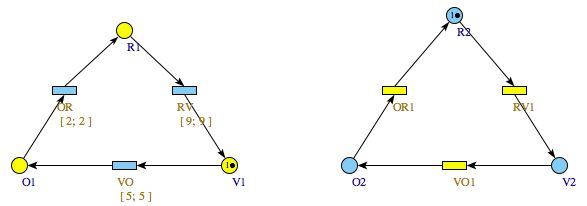
\includegraphics[scale=0.5]{ressources/part1/Q2.png}
	\caption{Réseau de Pétri, feux non synchronisés}
\end{figure}

Chaque feu est identique et dispose de trois places suivant les trois couleurs qu'un feu de circulation tricolore peut prendre: Rouge, Orange et Vert.

%%%%%%%%%%%%%%%%%%%%%%%
\subsection{Question 3}
%%%%%%%%%%%%%%%%%%%%%%%

\href{https://github.com/masters-info-nantes/hong-cheng-lv/blob/master/ressources/part1/Q3-FeuxSynchro.xml}{Feux
synchronisés et non temporises}

\begin{figure}[H]
	\centering
	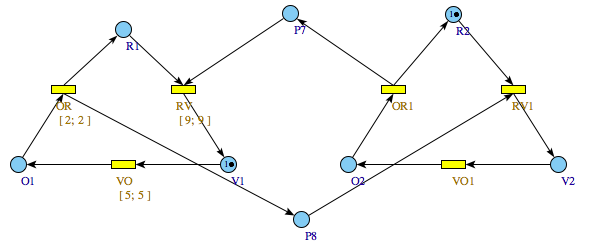
\includegraphics[scale=0.5]{ressources/part1/Q3.png}
	\caption{Réseau de Pétri, feux synchronisés}
\end{figure}

Dans le cas réel, les feux de circulation sont synchronisés. En effet, lorsqu'un premier feu est Vert, le second est Rouge. Puis le premier feu passe alternativement au Orange puis au Rouge tandis qu'ensuite le second feu devient Vert.

Pour respecter ce cahier des charges, nous avons ajouté deux places entre les deux feux. Alors, lorsqu'un feu devient Vert, il empêche l'autre de devenir Vert puis le libère une fois qu'il est passé à l'Orange puis au Rouge.

%%%%%%%%%%%%%%%%%%%%%%%
\subsection{Question 4}
%%%%%%%%%%%%%%%%%%%%%%%

Un graphe de marquage permet de montrer les différentes executions possibles de notre système de réseaux de Pétri.

\begin{figure}[H]
  \centering
  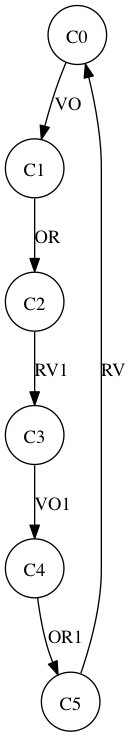
\includegraphics[scale=0.5]{ressources/part1/traitement-question4/graphe.png}
  \caption{Graphe de marquage des feux synchronisés}
\end{figure}

On constate que l'execution de notre système est linéaire. Cela signifie qu'il existe une seule execution, ainsi prouver que celle-ci est correcte revient à prouver que le système entier est correct.

%%%%%%%%%%%%%%%%%%%%%%%
\subsection{Question 5 et 6}
%%%%%%%%%%%%%%%%%%%%%%%

Vérification des propriétés de sureté et de vivacité du système de feux synchronisés.

\begin{itemize}
	\item Il y a toujours au minimum un feu rouge (sureté)
\begin{verbatim}
AG[0, inf](M(R1) + M(R2) >= 1)
\end{verbatim}

	\item Le deuxième feu passe au moins une fois au vert (non bloqué)
\begin{verbatim}
AG[0, inf](M(V2) = 1)
\end{verbatim}

	\item Les feux ne se bloquent pas entre eux
\begin{verbatim}
AG[0, inf](M(R1) + M(P7) = 2) # P7 = place intermédiaire
\end{verbatim}
\end{itemize}

\newpage
%%%%%%%%%%%%%%%%%%%%%%%%%%%%%%%%%%%%%%%%%%%%
\section{Partie 2 - Deux feux temporises}
%%%%%%%%%%%%%%%%%%%%%%%%%%%%%%%%%%%%%%%%%%%%
La partie précédente expose un système de feux synchronisés mais non temporises. En effet, dans la réalité les feux restent un temps donné dans leurs états. Nous proposons alors un système de feux temporises sous la forme d'automates à états finis modélisés avec le logiciel Uppaal.

%%%%%%%%%%%%%%%%%%%%%%%
\subsection{Question 7}
%%%%%%%%%%%%%%%%%%%%%%%

\href{https://github.com/masters-info-nantes/hong-cheng-lv/blob/master/ressources/part2/Q7-FeuxTemporises.xml}{Feux temporisés sans synchronisation}

\begin{figure}[H]
    \begin{minipage}[c]{.46\linewidth}
		\centering
		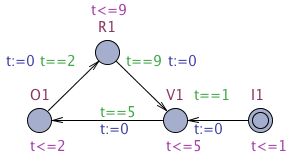
\includegraphics[scale=0.5]{ressources/part2/Q7-1.png}
		\caption{Automate du feu commençant en Vert}
    \end{minipage}
    \hfill%
    \begin{minipage}[c]{.46\linewidth}
		\centering
		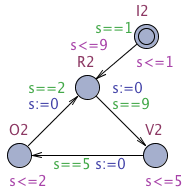
\includegraphics[scale=0.5]{ressources/part2/Q7-2.png}
		\caption{Automate du feu commençant en Rouge}
    \end{minipage}
\end{figure}

Par défaut, les automates ne démarrent pas en même temps et on observe une désynchronisation des feux. Une solution est d'ajouter un état avant l'état réel pour chacun des feux.


\subsection*{Validation des propriétés de sureté de vivacité du système de feux temporises.}

\begin{itemize}
	\item Toujours au moins un feu rouge
\begin{verbatim}
A[](feu1.R1 or feu2.R2 or feu1.I1 or feu2.I2)
\end{verbatim}

	\item Les deux feux atteignent leur état le plus éloigné, ils ne sont pas bloqués par le temps
\begin{verbatim}
E<>(feu1.R1 and feu2.02)
\end{verbatim}

	\item Pas de blocage
\begin{verbatim}
E<> deadlock
\end{verbatim}

\end{itemize}

%%%%%%%%%%%%%%%%%%%%%%%
\subsection{Question 8}
%%%%%%%%%%%%%%%%%%%%%%%

Afin de controller au mieux le système, cette solution propose l'utilisation d'un contrôleur.

Cet élément est chargé de faire évoluer les états des feux de manière correcte. Cela signifie par exemple qu'il lui est impossible de mettre les deux feux Verts en même temps.

\begin{figure}[h]
    \begin{minipage}[c]{.46\linewidth}
		\centering
		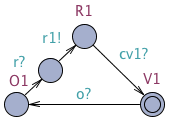
\includegraphics[scale=0.5]{ressources/part2/Q8-1.png}
		\caption{Automate du feu commençant en Vert}
    \end{minipage}
    \hfill%
    \begin{minipage}[c]{.46\linewidth}
		\centering
		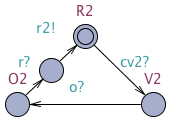
\includegraphics[scale=0.5]{ressources/part2/Q8-2.png}
		\caption{Automate du feu commençant en Rouge}
    \end{minipage}
\end{figure}

\begin{figure}[H]
	\centering
	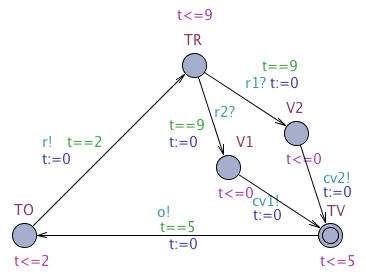
\includegraphics[scale=0.5]{ressources/part2/Q8-3.png}
	\caption{Contrôleur des feux}
\end{figure}

Les feux ne sont pas temporises mais il y a toujours un feu Rouge et un feu Vert au démarrage du système. En effet, c'est le rôle du contrôleur qui temporise et commande les feux à travers une synchronisation par signaux.

Le contrôleur allume alors alternativement le premier et le second feu tout en prenant en compte le temps pendant lequel chaque feu doit rester dans un état donné.

\subsection*{Vérification des propriétés de sureté de vivacité du système de feux synchronisés}

\begin{itemize}
	\item Toujours au moins un feu rouge
\begin{verbatim}
A[](feu1.R1 or feu2.R2)
\end{verbatim}

	\item Les deux feux atteignent leur état le plus éloigné, ils ne sont pas bloqués par le temps
\begin{verbatim}
E<>(feu1.R1 and feu2.O2)
\end{verbatim}

	\item Pas de deadlock
\begin{verbatim}
E<> deadlock
\end{verbatim}

\end{itemize}

%%%%%%%%%%%%%%%%%%%%%%%%%%%%%%%%%%%%%%%%%%%%
\section{Partie 3 - Carrefour en T}
%%%%%%%%%%%%%%%%%%%%%%%%%%%%%%%%%%%%%%%%%%%%
Après avoir étudié des systèmes représentant la synchronisation de deux feux de circulation sur une route, nous allons nous intéresser à un carrefour en T.

Comme dans le premier cas, il y a une route principale avec deux feux tricolores. On ajoute ici une route secondaire sur le côté. Dans un cas normal, le feux de la route secondaire est Rouge mais lorsque des voitures sont captés il passe au Vert.

%%%%%%%%%%%%%%%%%%%%%%%
\subsection{Question 9}
%%%%%%%%%%%%%%%%%%%%%%%

Dans cette première version de notre système de feux, il n'y a pas de contraintes de temps.

\begin{itemize}
	\item Les 2 feux de la route principale sont considérés comme un seul
	\item Il existe un processus qui régule l'arrivée des voitures dans la petite rue
\end{itemize}

\begin{figure}[H]
	\centering
	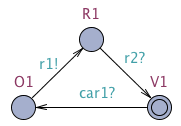
\includegraphics[scale=0.5]{ressources/part3/Q9-1.png}
	\caption{Automate du feu de la route principale}
\end{figure}

Le feu de la route principale passe du Vert au Orange, puis au Rouge lorsqu'un véhicule arrive sur la route secondaire. Il attend que le feu de la route secondaire soit Rouge et indique que les voitures de la route secondaires sont bien passées.

\begin{figure}[h]
    \begin{minipage}[c]{.46\linewidth}
		\centering
		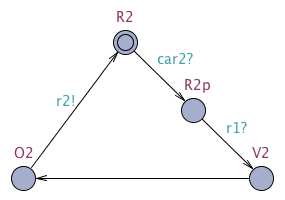
\includegraphics[scale=0.5]{ressources/part3/Q9-2.png}
		\caption{Automate du feu de la route secondaire}
    \end{minipage}
    \hfill%
    \begin{minipage}[c]{.46\linewidth}
		\centering
		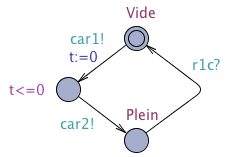
\includegraphics[scale=0.5]{ressources/part3/Q9-3.png}
		\caption{Automate de l'arrivée des véhicules sur la route secondaire (capteur)}
    \end{minipage}
\end{figure}

Par défaut Rouge, le feu de la route secondaire passe au Vert si une voiture est détectée et que les feux de la route principale sont Rouges.

L'automate qui conditionne l'arrivée des voitures sur la route secondaire est réprésenté par deux états principaux: route vide et route plein (présence d'une voiture au moins). Le signal \emph{r1c} permet d'assurer que la voiture détectée sur la route secondaire soit bien passée pendant que le feu était Vert.

%%%%%%%%%%%%%%%%%%%%%%%
\subsection{Question 10}
%%%%%%%%%%%%%%%%%%%%%%%

A notre système de feux sur un carrefour en T, nous ajoutons ici des contraintes de temps notamment sur le temps pendant lequel chaque feu doit rester Vert.

\begin{itemize}
	\item Le feu de la route secondaire reste Vert pendant 30 secondes
	\item Dans un cycle, le feu de la route principale doit être Vert pendant au moins 30 secondes
	\item Chaque feu reste orange pendant 5 secondes
\end{itemize}

\begin{figure}[H]
	\centering
	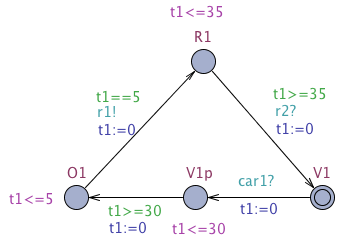
\includegraphics[scale=0.5]{ressources/part3/Q10-1.png}
	\caption{\label{fig:majorRoadQ10}Automate du feu de la route principale}
\end{figure}

Les signaux \emph{r1} et \emph{r2} permettent d'obliger qu'un des feux soit rouge à n'importe quel moment.

Le feu de la route principale attend qu'une voiture arrive sur la route secondaire pour passer à l'Orange. Attention, le feu respecte aussi le fait qu'il doit rester au Vert eu moins 30 secondes même si une voiture est détectée avant.

Avant de repasser au Vert, le feu de la route principale attend que celui de la route secondaire soit passé au Rouge.

\begin{figure}[H]
    \begin{minipage}[c]{.46\linewidth}
		\centering
		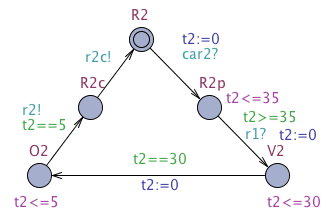
\includegraphics[scale=0.5]{ressources/part3/Q10-2.png}
		\caption{\label{fig:minorRoadQ10}Automate du feu de la route secondaire}
    \end{minipage}
    \hfill%
    \begin{minipage}[c]{.46\linewidth}
		\centering
		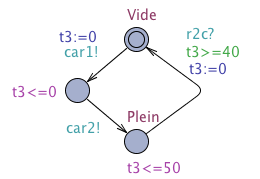
\includegraphics[scale=0.5]{ressources/part3/Q10-3.png}
		\caption{\label{fig:roadSyncQ10}Automate de l'arrivée des véhicules sur la route secondaire (capteur)}
    \end{minipage}
\end{figure}

Pour passer au Vert, le feu de la route secondaire doit l'arrivée d'une voiture mais aussi que le feu de la route principale soit Rouge.

Les signaux \emph{car1} et \emph{car2} permettent d'indiquer au feu de la route principale et au feu de la route secondaire qu'une voiture est arrivée sur la route secondaire. Le feu de la route principale notifie aussi l'automate d'arrivée des véhicules pour indiquer que la voiture est passée.

%%%%%%%%%%%%%%%%%%%%%%%
\subsection{Question 11}
%%%%%%%%%%%%%%%%%%%%%%%

%%%%%%%%%%%
\subsubsection{Validations question 9}
%%%%%%%%%%%

\begin{itemize}
	\item Toujours au moins un feu rouge
\begin{verbatim}
A[](Major.R1 or Major.R1c or Minor.R2 or Minor.R2p)
\end{verbatim}

	\item Lorsque le feu de la route secondaire passe au vert, il doit y avoir au moins une voiture qui passe sur la route secondaire.
\begin{verbatim}
E<>(Car.Vide and Minor.V2)
\end{verbatim}

	\item Les deux feux atteignent leur état le plus éloigné, ils ne sont pas bloqués
\begin{verbatim}
E<>(Major.R1 and Minor.O2)
\end{verbatim}

	\item Pas de deadlock
\begin{verbatim}
E<> deadlock
\end{verbatim}

\end{itemize}

%%%%%%%%%%%
\subsubsection{Validations question 10}
%%%%%%%%%%%

\begin{itemize}
	\item Toujours au moins un feu rouge
\begin{verbatim}
A[](Major.R1 or Major.R1c or Minor.R2 or Minor.R2p)
\end{verbatim}

	\item Lorsque le feu de la route secondaire passe au vert, il doit y avoir au moins une voiture qui passe sur la route secondaire.
\begin{verbatim}
E<>(Car.Vide and Minor.V2)
\end{verbatim}

	\item Les deux feux atteignent leur état le plus éloigné, ils ne sont pas bloqués par le temps
\begin{verbatim}
E<>(Major.R1 and Minor.O2)
\end{verbatim}

	\item Pas de deadlock
\begin{verbatim}
E<> deadlock
\end{verbatim}
\end{itemize}

%%%%%%%%%%%%%%%%%%%%%%%%%%%%%%%%%%%%%%%%%%%%
\section{Implémentation}
%%%%%%%%%%%%%%%%%%%%%%%%%%%%%%%%%%%%%%%%%%%%

\begin{figure}[H]
  \centering
  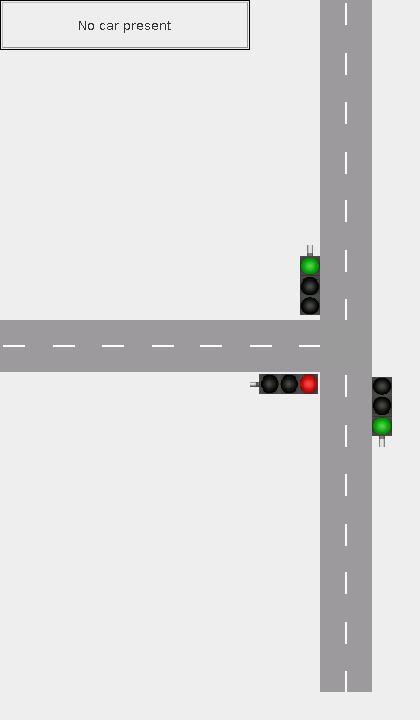
\includegraphics[width=8cm, angle=90]{ressources/impl/Tjunction.png}
  \caption{\label{fig:screenshot} Interface du carrefour en T}
\end{figure}


Notre implémentation simule un carrefour en T présenté par les figures \ref{fig:majorRoadQ10} et \ref{fig:minorRoadQ10}, synchronisé par la figure \ref{fig:roadSyncQ10}.

On a utilisé un Thread par feu (class Road) pour l'autonomie et l'indépendance.
On a une classe (Tjonction) qui sert de contrôleur pour synchroniser les feux.

Chaque route a deux procédures pour passer au rouge ou pour passer au vert. Le contrôleur permet de faire passer le signal au principal que la route secondaire à besoin de passer au vert, mais aussi permettre de temporiser les feux pour avoir une équité entre les deux routes.

Dans notre interface, nous simulons la présence de voiture par le bouton à deux états.
Un état pour indiquer quand une voiture est présent sur la route secondaire, un deuxième état pour indiquer qu'il n'y a aucun voiture.


\end{document}
